\chapter*{Úvod}
\addcontentsline{toc}{chapter}{Úvod}
Už v antike sa niektorí antickí filozofi zaoberali myšlienkou, že základná charakteristika jednotlivých biologických druhov sa časom mení.
A práve v gréčtine môžeme nájsť pôvod slova \emph{Fylogenéza}, kde fylé = kmeň a genesis = zrodenie/pôvod.
Fylogenéza sa zaoberá vývojom druhu organizmov. Väčšinou sa odohráva počas veľmi dlhého časového úseku, 
a preto ju nie sme schopní priamo pozorovať a nezostáva nám iná možnosť ako vytvoriť rekonštrukciu na základe poznatkov o evolúcii.
Neskôr v tomto vednom poli urobil významný pokrok Charles Darwin, keď v roku 1859 publikoval svoju knihu \emph{Pôvod druhov}.
Okrem toho, že z evolúcie vytvoril široko uznávanú teóriu, predstavil aj myšlienku že akékoľvek dva veľmi rozdielne
druhy zdieľajú spoločného predka a vizuálne ju znázornil vo forme stromového grafu, takzvaného \emph{stromu života}.
Tak položil základy Evolučnej teórie, ktorá skúma evolučné procesy, ktoré
na zemi vytvorili rôznorodosť života z počiatočnej živej formy. 
Ďalšie poznatky v oblasti genetiky, súvisejúce s DNA a RNA viedli k tomu, že na evolúciu sa
dnes pozeráme hlavne prostredníctvom génov.
Sekvenovanie DNA umožnilo vzťahy medzi jednotlivými organizmami odsledovať na základe zmien, ktoré prebehli v ich DNA sekvencii.
To nám ponúka množstvo presných dát využiteľných pri rekonštrukcii fylogenetického procesu.
Aj na našej fakulte vzniklo niekoľko prác, ktoré sa venujú rekonštrukcii DNA sekvencie pokiaľ poznáme jej súčasný vzhľad,
prípadne sa snažia zrekonštruovať fylogenetický strom pokiaľ poznáme DNA sekvencie súčasných druhov 
\cite{Kovac2011,Hozza2014,Herencsar2014,Vinar2010}. 
\begin{figure}[t]
 \centering
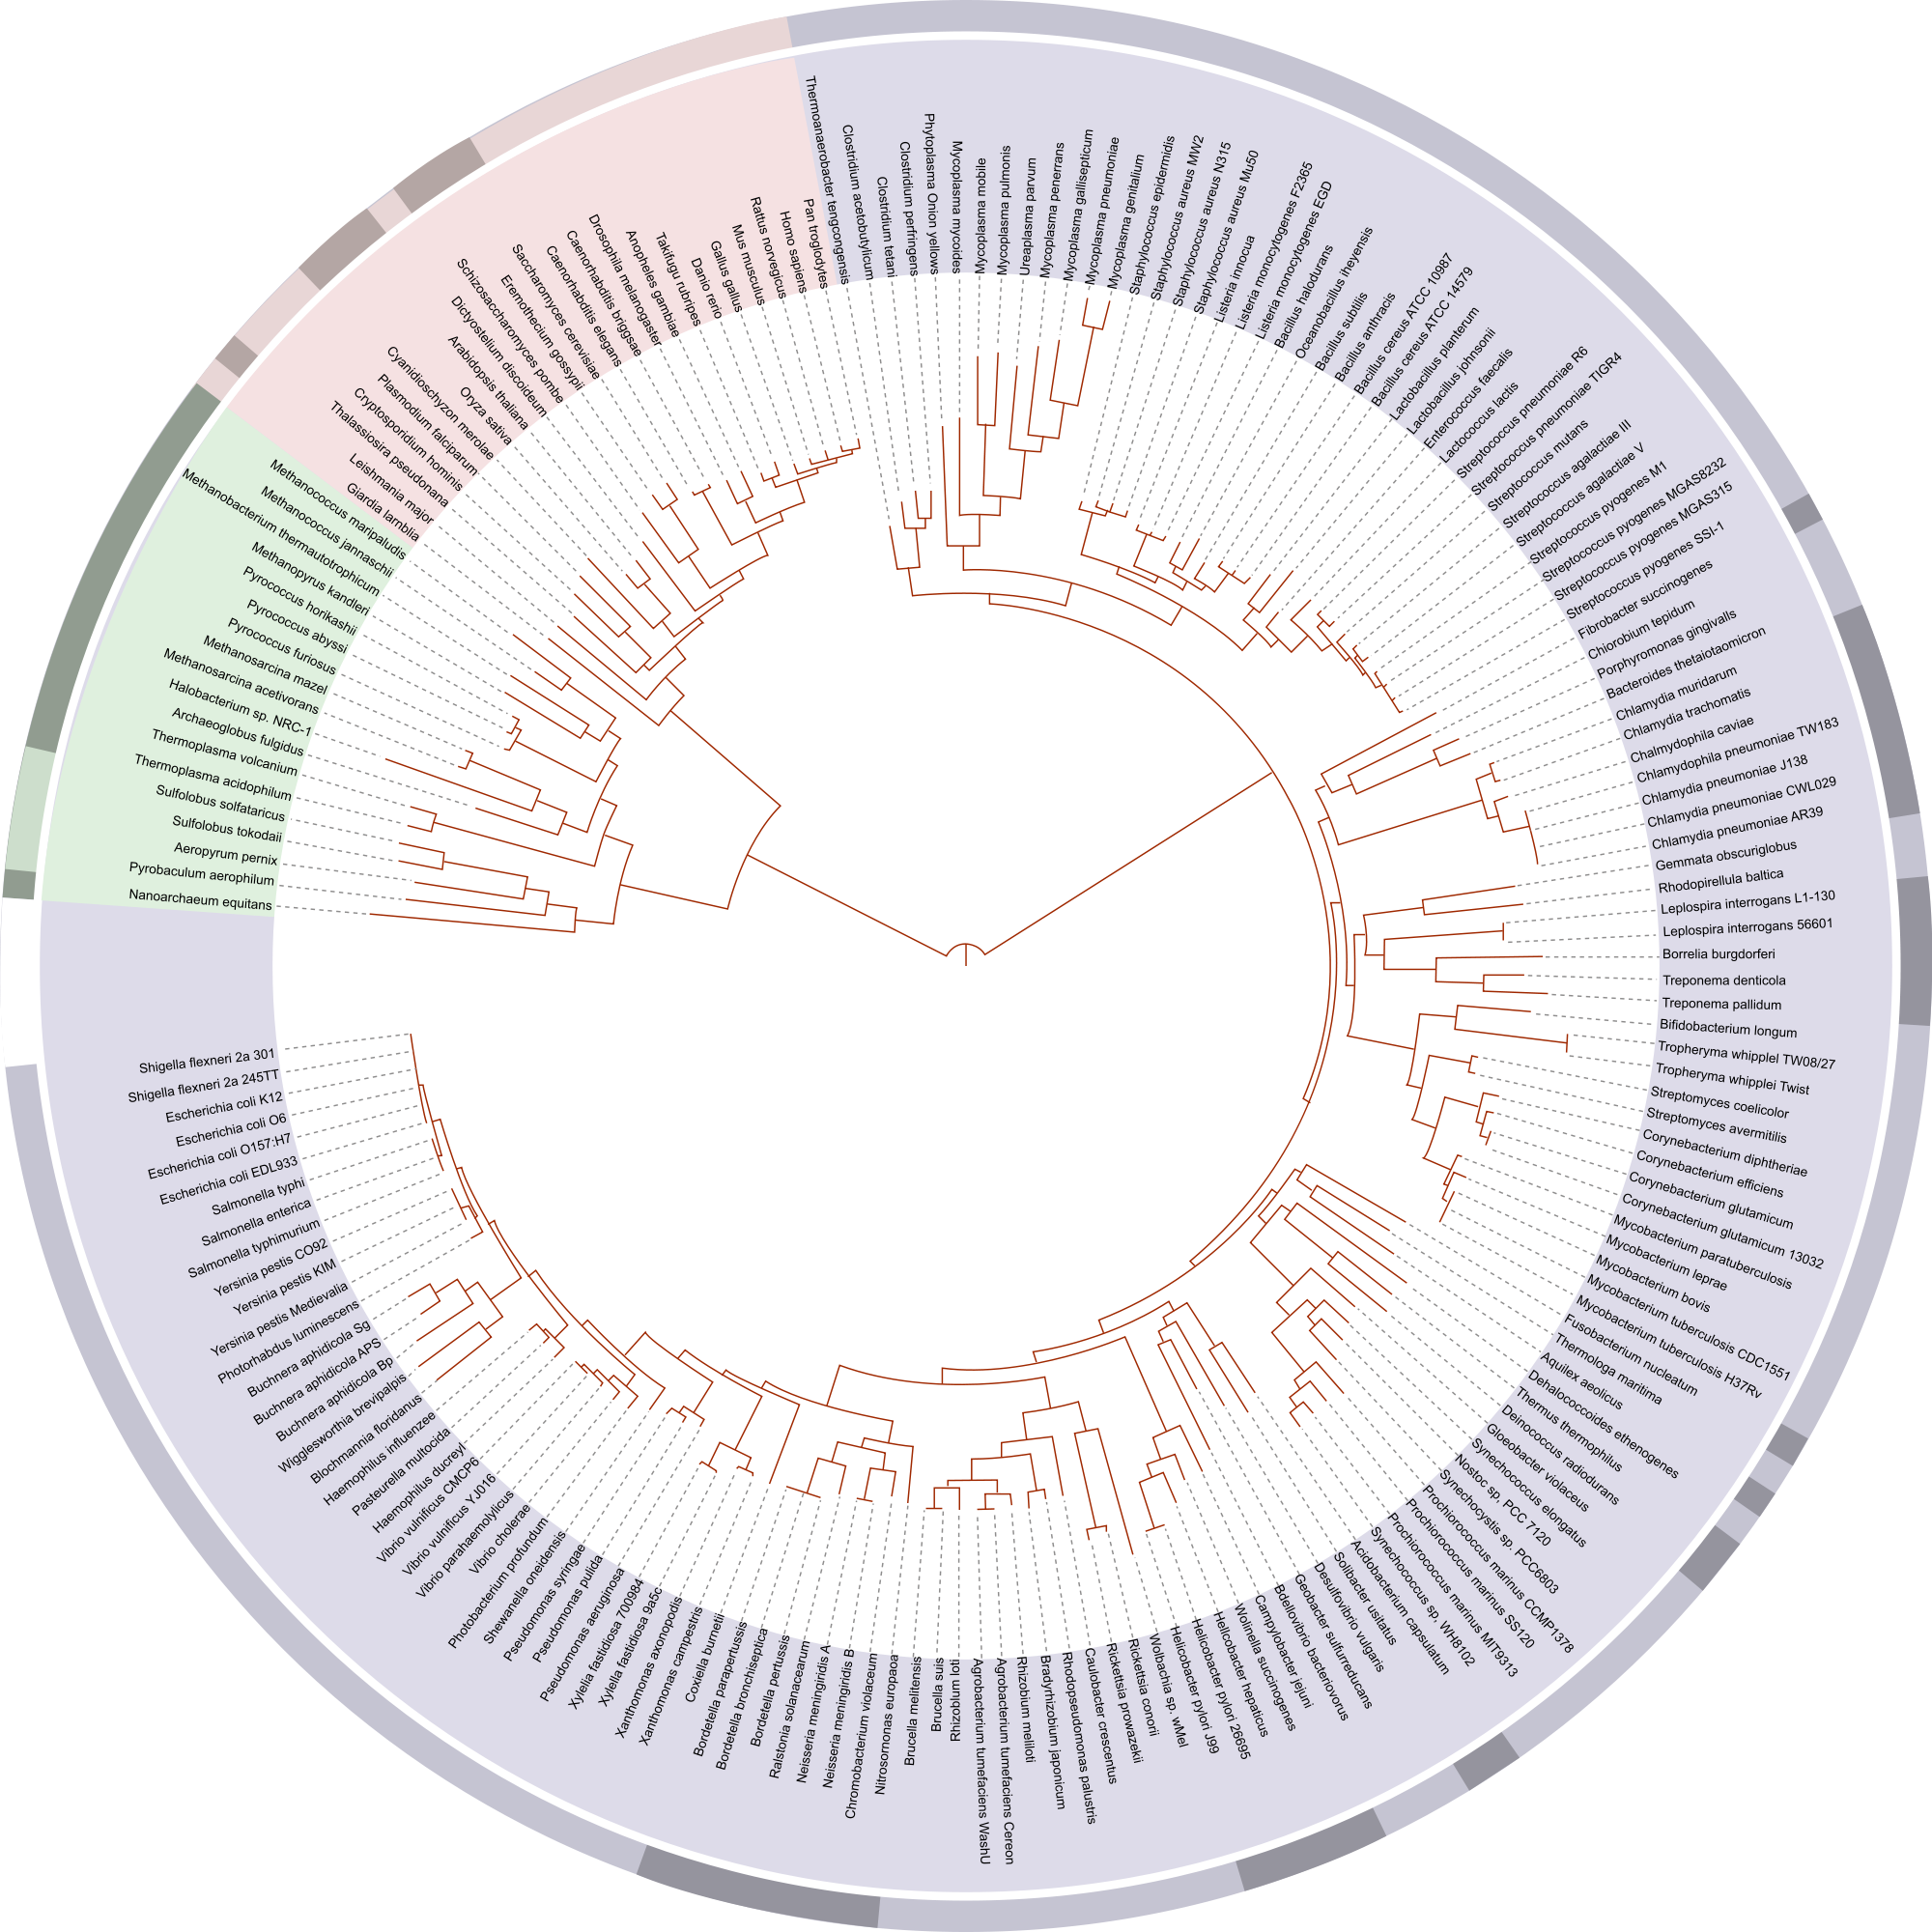
\includegraphics[width=1\textwidth]{images/tol}
\caption{Fylogenetický strom zobrazujúci evolučné vzťahy veľkého počtu druhov. Zdroj: wikipedia.org}\label{obr:tol}
\end{figure}

Strom stále patrí medzi najpopulárnejšie spôsoby ako zobraziť evolučné vzťahy medzi druhmi alebo inými objektami.
Najčastejšie sa stretávame s fylogenetickým stromom, ktorý zobrazuje vývoj druhov z posledného spoločného predka, ako napríklad vidíme na obrázku \ref{obr:tol}.
V takomto zobrazení nevidno samotné zmeny DNA, informácie, ktoré nám poskytnú, 
ako napríklad vzdialenosť dvoch objektov na základe rozdielnosti ich DNA sekvencie, však bývajú použité na zostavenie stromu.
Cieľom tejto práce je zostrojiť program, ktorý zobrazí jednoduchú postupnosť sekvencií DNA s dôrazom na zmeny, ktoré sa udiali s génmi v týchto sekvenciách.
Výsledok by mal predstavovať malú vetvu fylogenetického stromu, v ktorom prepojenie objektov zobrazí reálne zmeny, ktoré sa odohrali na ich DNA sekvencii.
Inšpiráciou pre túto prácu sú vyššie spomenuté práce pochádzajúce z našej fakulty,
náš program má byť schopný vizualizovať výsledky, ktoré produkujú a poslúžiť okrem iného ako rýchla optická kontrola správnosti.

Prvá kapitola poskytne úvod do problematiky, predstavíme si základné biologické a bioinformatické pojmy, potrebné pre našu prácu.
Druhá kapitola sa bude venovať implementácii nášho programu \emph{EHDraw},popíšeme ako vyzerá jeho vstup a výstup,
aké možnosti interakcie poskytuje používateľovi a ktoré nastavenia v ňom vieme meniť.
Okrem základnej funkcionality súvisiacej so zobrazovaním evolučnej histórie, sme sa zamerali na problém,
ako zredukovať množstvo zobrazených génov. Naším cieľom je odstrániť niektoré gény tak, aby sa výsledný obrázok stal prehľadnejším, 
a aby v ňom zostali zachované informácie o udalostiach, ktoré sa nachádzajú v evolučnej histórii.
Tretia kapitola popisuje, ako problém výberu takýchto génov pretransformujeme na \emph{Problém množinového pokrytia},
ako aj dve metódy ktorými budeme \emph{Problém množinového pokrytia} riešiť. Konkrétne sa jedná o greedy algoritmus, ktorý nájde aproximačné riešenie,
a Celočíselné lineárne programovanie, ktorým hľadáme optimálne riešenie.
Štvrtá kapitola nadväzuje na tretiu, porovnávame v nej, aké výsledky dostaneme v závislosti od toho, akú metódu výberu génov zvolíme,
a v ktorých prípadoch dochádza k najväčšej redukcii množstva zobrazených génov. 
